%%%%%%%%%%%%%%%%%%%%%%%%%%%%%%%%%%%%%%%%%%%%%%%%%%%%%%%%%%%%%%%%%%%%%%%%%%%%%%%%
%	TRABAJO: Proyecto Integrador
%		Titulo: 	Desarrollo de IP cores con procesamiento de Redes de Petri 	
%					Temporales para sistemas multicore en FPGA					
%		Autores:	Juli�n Nonino												%					Carlos Renzo Pisetta										%		Director:	Orlando Micolini											
%%%%%%%%%%%%%%%%%%%%%%%%%%%%%%%%%%%%%%%%%%%%%%%%%%%%%%%%%%%%%%%%%%%%%%%%%%%%%%%%

% Path im�genes: ./desarrollo/implementacion_FPGA/img
% Nombre predeterminado im�genes: implexx
%	xx es el numero de imagen

\section{F�brica de mesas}
	\label{sec:fabrica_mesas}
	
	En este caso, se modelar� de manera sencilla el proceso de fabricaci�n de una mesa. Modelando el problema con Redes de Petri, y contando con un procesador capaz de ejecutarlas, podemos validar y verificar las propiedades del modelo y luego, asegurar que la implementaci�n del programa satisface las mismas propiedades del modelo.
	\begin{figure}[H]
		\centering
		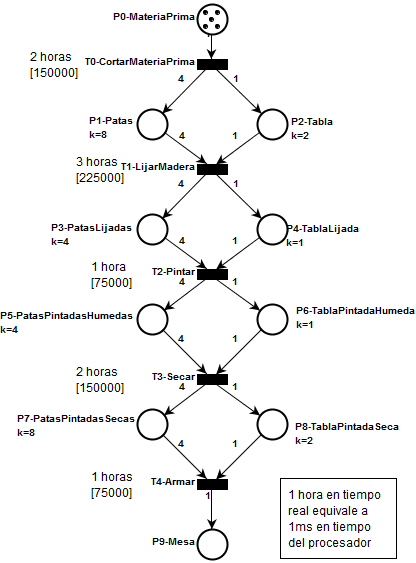
\includegraphics[width=0.75\linewidth,keepaspectratio]{./desarrollo/implementacion_FPGA/img/imple04}
		\caption{Red de Petri que modela una f�brica de mesas}
		\label{fig:imple04}
	\end{figure}
	
	\newpage
	
	Utilizando el software PIPE, se efectuaron ciertos an�lisis sobre la Red de Petri obteniendo los siguientes resultados.
	\begin{figure}[H]
		\centering
		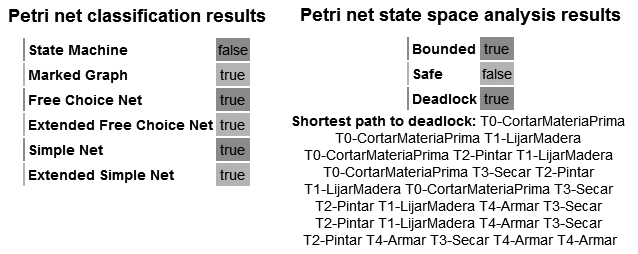
\includegraphics[width=1\linewidth,keepaspectratio]{./desarrollo/implementacion_FPGA/img/imple05}
		\caption{Clasificaci�n y an�lisis del espacio de estados de la Red de Petri}
		\label{fig:imple05}
	\end{figure}
	
	De la Figura \ref{fig:imple05} se observa que la Red de Petri tiene restricciones en su sintaxis, lo cual, produce que sea clasificada como una grafo de marcado. Esto significa, que todas sus plazas tienen un �nico arco de entrada y/o un �nico arco de salida. El an�lisis del espacio de estados de la red que modela el problema planteado, muestra que es una red limitada pero, no es una red segura. Adem�s, con este an�lisis, se descubre que la red de Petri tiene un estado de deadlock, la plaza \emph{P9}. Es decir, la Red de Petri, en alg�n momento se detiene, deja de estar activa.
	\\
	
	Para ejecutar la red se instanci� en la FPGA el Procesador de Petri con el agregado de interrupciones para todas las transiciones, de manera que los hilos se duerman para esperar la ejecuci�n de su disparo en vez de preguntar constantemente ya que �stas, no se ejecutar�n hasta que transcurra el tiempo m�nimo en que puede ser disparada la transici�n sensibilizada.
	\\

	Se desarroll� un programa en \emph{C} que carga los valores necesarios en el procesador para ejecutar la red. Luego $5$ hilos encargados cada uno de una actividad distinta piden y retiran el disparo de una transici�n determinada. Una vez terminan la tarea informan de esto mediante consola escribiendo el numero de mesa en el cual estaban trabajando. Este programa, puede encontrarse en la secci�n \ref{sec:programa_fabrica_mesas_petri}.
	
	\newpage

	Al ejecutar el programa, se obtiene el siguiente resultado.
	\begin{verbatim}
Comienza la Carga de la Matriz de Incidencia
Termino Carga de la Matriz de Incidencia 

Comienza la Carga de la Matriz de Inhibicion
Termino Carga de la Matriz de Inhibicion

Comienza la Carga del vector de Cotas de Plazas 
Termino Carga del vector de Cotas de Plazas

Comienza la Carga del vector de Transiciones Automaticas
Termino Carga del vector de Transiciones Automaticas

Comienza la Carga del vector EFT
Termino Carga del vector de EFT

Comienza la Carga del vector de incrementos
Termino Carga del vector de incrementos

Comienza la Carga del vector LFT
Termino Carga del vector de LFT

Comienza la Carga del vector de Marcado Inicial
Termino Carga del vector de Marcado Inicial

Comienza la Carga del vector de Transiciones con Interrupcion
Termino Carga del vector de Transiciones con Interrupcion

Semaforos creados correctamente

Mesa 1: CORTADA
Mesa 2: CORTADA
Mesa 1: LIJADA
Mesa 1: PINTADA
Mesa 1: SECADA
Mesa 3: CORTADA
Mesa 2: LIJADA
Mesa 2: PINTADA
Mesa 2: SECADA
Mesa 1: ARMADA
Mesa 4: CORTADA
Mesa 3: LIJADA
Mesa 3: PINTADA
Mesa 3: SECADA
Mesa 2: ARMADA
Mesa 5: CORTADA
Mesa 4: LIJADA
Mesa 4: PINTADA
Mesa 4: SECADA
Mesa 3: ARMADA
Mesa 5: LIJADA
Mesa 5: PINTADA
Mesa 5: SECADA
Mesa 4: ARMADA
Mesa 5: ARMADA
SE ARMARON 5 MESAS

TODOS LOS HILOS TERMINARON	
	\end{verbatim}
	
